%!TEX root=seke.tex
% mainfile: seke.tex

\documentclass[10pt,twocolumn]{article}

\usepackage[table]{xcolor}% http://ctan.org/pkg/xcolor
\usepackage{latex8}
\usepackage{times}
\usepackage{inconsolata}
\usepackage{pifont}

\usepackage{graphicx}
\usepackage{algorithm}
\usepackage{algorithmic}

\usepackage{tikz}
\usetikzlibrary{shapes,arrows,shadows}
\usepackage{amsmath,bm,times}
\usepackage{verbatim}

\usepackage{subcaption}
\usepackage{fancyhdr}
\renewcommand{\headrulewidth}{0pt}
\fancypagestyle{doi}{\lfoot{DOI reference number: placeholder}}

\usepackage[small,compact]{titlesec}

\usepackage{listings}

\pagenumbering{gobble}

\newcommand{\goallegheny}{$^{\mbox{\footnotesize \ding{72}}}$}
\newcommand{\gosheffield}{$^{\mbox{\footnotesize \ding{73}}}$}
\newcommand{\gospace}{$\;$}


\begin{document}


\title{\vspace*{-.6in}Assignment2 Neural Network\vspace*{-.1in}}
\author{
	Zihe Liu
}
\affiliation{
 	1831581
}
\maketitle



\section{Introduction}
We implement the Neural Network based on Python and numpy, and train and evaluate model on two data sets including iris and wine-quality.

\section{Environment}
\vspace*{-.05in}

The version of Python requires as least 3.5. Run the following command in the shell to install third party dependencies.
\begin{lstlisting}[language=bash]
$ pip install -r requirements
\end{lstlisting}

To train the Neural Network, we can run the command "python train.py" with the arguments in the Table \ref{table:command}.
\begin{table*}[hbt]
	\caption{The arguments for train.py}
	\label{table:command}
	
	\centering
	\begin{tabular}{l|l|l}		
		Arguments		&Introduction								&Type \\ \hline
		prefix	 		&The prefix of data set path	.				&str	 \\
		hidden\_sizes 	&The hidden size of each hidden layer.		&multiple numbers spitted by ','. Eg: '12,12,12' \\
		batch\_size	 	&The size of batch.							&int, default is 8 \\
		learning\_rate	&The learning rate							&float, default is 0.01 \\
		activator		&The activator of hidden size				&'sigmoid' or 'tanh'
	\end{tabular}
\end{table*}
For example, the following command is to train Neural Network on iris data set with specific hyper parameters.
\begin{lstlisting}[language=bash]
$ python train.py \
    --prefix=static/input/iris/iris \
    --hidden_sizes=32 \
    --learning_rate=0.01 \
    --batch_size=8 \
    --activator=tanh                 
\end{lstlisting}


\section{Data Set and Data Preprocessing}
We choose two data sets to train Neural Network, including iris and abalone.The iris data set has 150 instances, 4 features and 3 categories. And the abalone data set has 4117 instances, 8 features, and 29 categories.

\textbf{Reshuffle data set}. For each data set, we reshuffle the data set so that the model can learn more general features from it. 



\begin{figure}[tb]
	\centering
	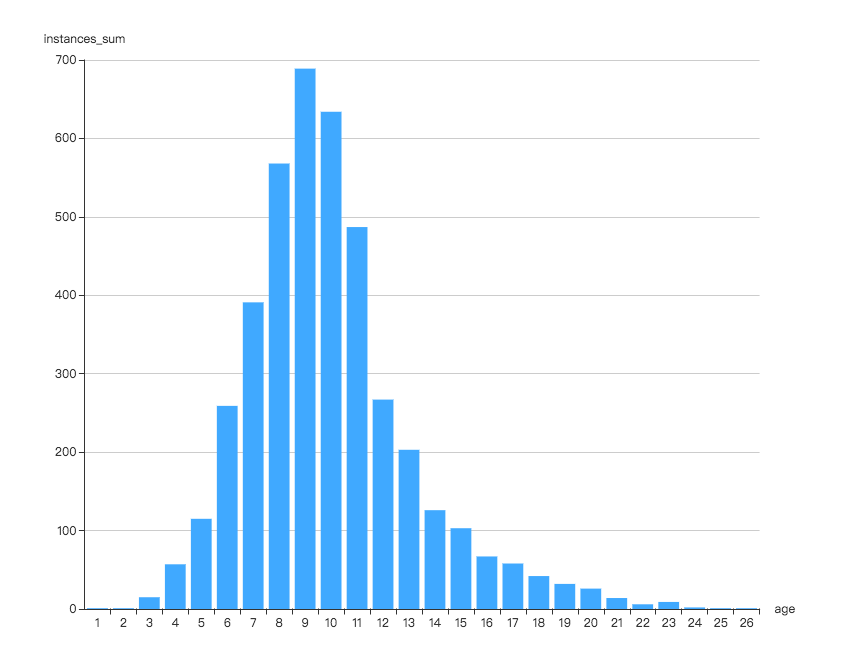
\includegraphics[width = .5\textwidth]{images/age-dis.png}
	\caption{The histogram on classification and its number of instances on abalone data set.}
	\label{fig:age-dis}
\end{figure}

\textbf{Combine different categories}. As for abalone data set, there are 29 classifications and the histogram on classification and its number of instances is show as Figure \ref{fig:age-dis}. We can see four ages including 7, 8, 9 and 10 are far higher than others. It is so imbalance between different classification that the neural network can not well classify them. So we combine different categories to three categories: lower than 9, 9 and 10, bigger than 10. 

\textbf{Split train set, validation set and test set}. And we divide data set into train set, validation set and test set by 80\%, 10\% and 10\%. As the model optimizes the learnable parameters on the training set, the loss value on the training set is gradually reduced. But when the number iterations is too big, the model will learn the features specific to this training set but not universal features. As a result, the model is overfitting and accuracy decreases.

So we use training set and validation set to train model and decide whether to early stop. At each iteration, we firstly use training data set to optimize the model with SGD algorithm and respectively calculate average loss values of training data and validation data. If the average loss values of training data or validation data increases 5 times, which means loss value on validation data set has converged and will be overfitting if continue training, we early stop the training.
% \vspace*{-.05in}
\section{Program Modules}
\vspace*{-.05in}
There are 8 parts in out program, including \textsl{requirements.txt}, \textsl{model/}, \textsl{preprocess/}, \textsl{static/}, \textsl{utils/}, \textsl{constants.py}, \textsl{data.py} and \textsl{train.py}.

\subsection{requirements.txt}
The content of \textsl{requirements.txt} is the third-party dependencies and their version. This file is generated by the following command.
\begin{lstlisting}[language=bash]
$ pip freeze > requirements
\end{lstlisting}

\subsection{preprocess/}
The module \textsl{preprocess/} is to preprocess the raw data set into fixed formal file. Firstly it reshuffle the data set and then divide the raw data set into train, validation and test set by 80\%, 10\% and 10\%.

As the model optimizes the learnable parameters on the training set, the loss value on the training set is gradually reduced. But when the number iterations is too big, the model will learn the features specific to this training set but not universal features. As a result, the model is overfitting and accuracy decreases.

 So we use training set and validation set to train model and decide whether to early stop. At each iteration, we firstly use training data set to optimize the model with SGD algorithm and respectively calculate average loss values of training data and validation data. If the average loss values of training data or validation data increases 5 times, which means loss value on validation data set has converged and will be overfitting if continue training, we early stop the training.

\subsection{data.py}
\textsl{data.py} is to read the preprocessed data set and store \textsl{train\_source\_data}, \textsl{train\_target\_data}, \textsl{eval\_source\_data}, \textsl{eval\_target\_data}, \textsl{test\_source\_data} and \textsl{test\_eval\_data} in the instance of Class \textsl{Data}. Each instance of target data is an one hot vector full of zero except the position whose index is the relevant category. For example, if the category of a data instance is 2 with 4 categories in all instances, then the target data of this instance is [0, 0, 1, 0].

What's more, the class \textsl{Data} also provide methods to get batch data of train, validation and test sequentially. And there are also some methods to provide the common values such as \textsl{input\_size}, \textsl{output\_size} and \textsl{train\_batches\_sum}.

\subsection{constants.py}
\textsl{constants.py} stores the constant values used in project, including paths static files and suffix of fixed formal data set file. 

\subsection{utils/}
\textsl{utils/} has various tool methods. \textsl{file\_utils.py} is to transform between file and string, transform between JSON file and dict, and make directory if it does not exist. \textsl{log\_utils.py} is to output logs to the console and file. And \textsl{shell\_args.py} is to define the formate of arguments used in shell.

\subsection{model/}
The module \textsl{model/} defines the Neural Network model, with three parts including \textsl{activator/}, \textsl{fully\_connected\_layer.py} and \textsl{neural\_network.py}. 

All calculations in the model use matrix operations by \(numpy\) instead of loops in \(python\). Because matrix operations by \(numpy\) underlying layer is implemented in C++, which is much faster than \(python\).

\subsubsection{Neural Network Model}
\begin{figure}[htbp]
	\centering
	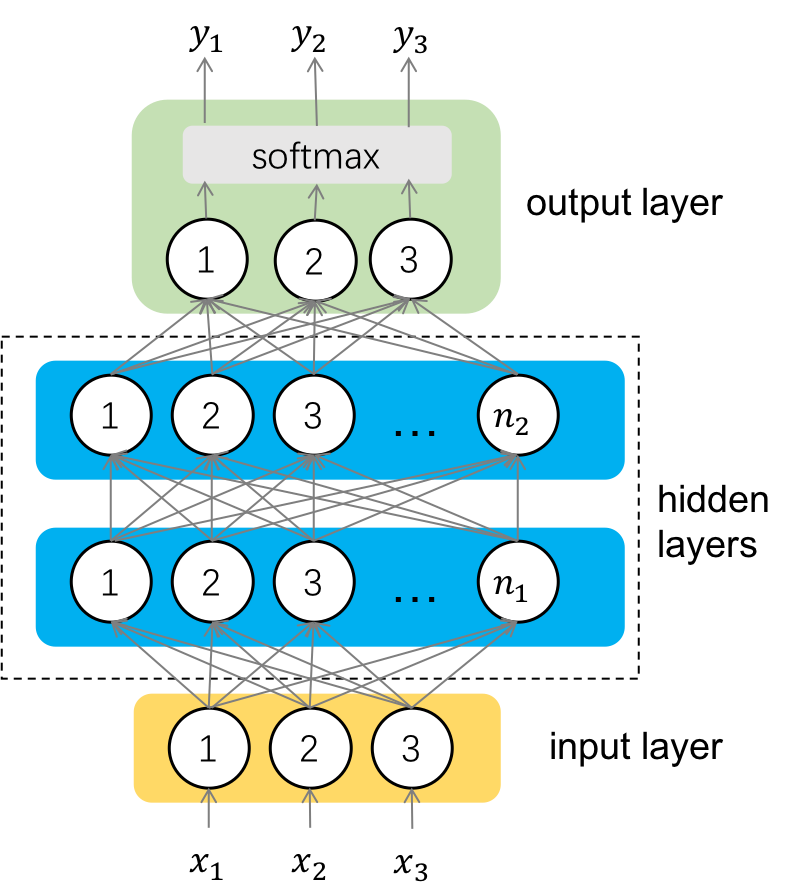
\includegraphics[width = .4\textwidth]{images/dnn.png}
	\caption{The overall structure of full connected Neural Network.}
	\label{fig:dnn}
\end{figure}

We implement the full connected Neural Network shown as Figure \ref{fig:dnn}. Neural networks are actually multiple neurons connected according to certain rules. There are one input layer, output layer, and multiple hidden layers between them.

The number of neurons in input layer is the number of features in source data. The number of neurons in output layer is the number of categories in target data. Each output of neuron in output layer represents the probability of getting this category based on the input features, which is between 0 and 1 and the sum is equal to 1.

For the \(i\)-th layer, the output vector is calculated by the following equation according to the input vector:
% equation for y_{i+1}
\begin{equation}
\boldsymbol{y_{i}} = f(\boldsymbol{x_{i}}\boldsymbol{w_i} + \boldsymbol{b_i})
\end{equation}
where \(\boldsymbol{y_{i}}\) is the output vector, \(\boldsymbol{x_{i}}\) is the input vector, \(\boldsymbol{w_{i}}\) and \(\boldsymbol{b_{i}}\) is the learnable parameters, and \(f\) is the activator function. The activator in output layer is \(softmax\) as follows:
% equation for softmax
\begin{equation}
softmax(z_k) = \frac{e^{z_k}}{\sum_{i=1}^{n}{e^{z_i}}}
\end{equation}
where \(n\) is the output size. Except output layer, the activator in each layer is \(sigmoid\) or \(tanh\) as follows.
% equation for softmax
\begin{equation}
sigmoid(z) = \frac{1}{1 + e^{-z}}
\end{equation}
% equation for tanh
\begin{equation}
tanh(x) = \frac{e^{x} - e^{-x}}{e^{x} + e^{-x}}
\end{equation}

The loss function is the cross entropy calculated by the negative log likelihood:
% equation for sigmoid
\begin{equation}
Loss = \frac{1}{m}\sum_{i=1}^{m}{-t_{i}{\rm log}y_i}
\end{equation}
where \(m\) is the number of categories, \(t_i\) is the target value and \(y_i\) is the predicted value for the category \(i\).

\subsubsection{The Module activator/}
There is a abstract class \(Activator\) with two abstract methods: \(forward\) which is used to calculate output by the input, \(backward\) which is used to calculate the derivative of the activator according to the output calculated by the \(forward\). And the subclass \(SoftmaxActivator\), \(SigmoidActivator\), \(TanhActivator\) respectively implement their respective \(backward\) and \(forward\).

\subsubsection{The Module fully\_connected\_layer.py}
The class \(FullyConnectedLayer\) is represented a layer in Neural Network. It stores and updates the learnable vector \(\boldsymbol{weights}\) and \(\boldsymbol{bia}\). It also provides how to initial the learnable vector such as full of zero, random uniform and random normal.

It provides methods \(forward\) to calculate the output vector according to input, weights, bia and activator, and \(backward\) to calculate the gradient delta according to the gradient of previous layer.
\subsubsection{The Module neural\_network.py}
The class NeuralNetwork define the structure of the model, including the input size, output size, number of hidden layer, the size of each hidden layer and the activator of each layer.

It also provides methods to train model with batch source data and relevant target data, predict category by the source data, and calculate the loss value according to source data and target data.

\subsection{train.py}
In this module, we train the Neural Network model using different data sets and hyper parameters. We use batch data to train the model, and use batch Stochastic Gradient Descent(SGD) algorithm to optimize the parameters of the  model. At each iteration, we firstly optimize the model on train data set and calculate the average loss value of it. Then we calculate the average loss value on validation data set without optimizing model. And if the loss value of train data or validation data increases more than 5 times, we early stop training.

After finishing training, respectively calculate accuracy rate in train data set, validation data set and test data set.

\subsection{static/}
The static directory stores the input data set, and output logs and figures.


\section{Evaluation of Results}\label{sec:evaluation}
We train the Neural Network model on iris data set and wine-quality data set. 

\begin{figure}[tbp]
	\centering
	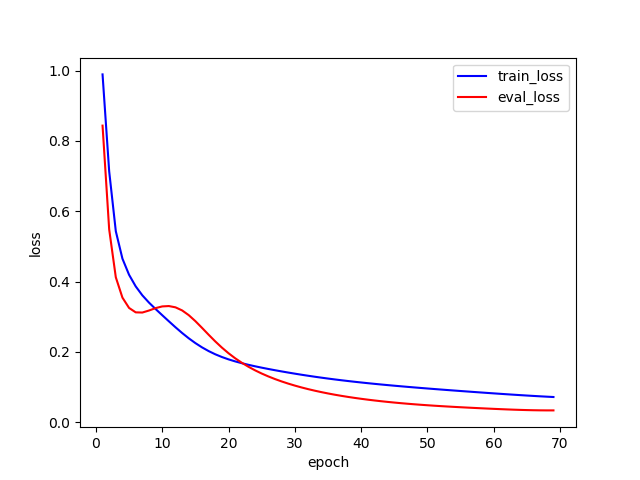
\includegraphics[width = .5\textwidth]{images/iris_loss.png}
	\caption{The epoch-loss curves for train data and validation data on iris data set.}
	\label{fig:iris_loss}
\end{figure}

\begin{figure}[tbp]
	\centering
	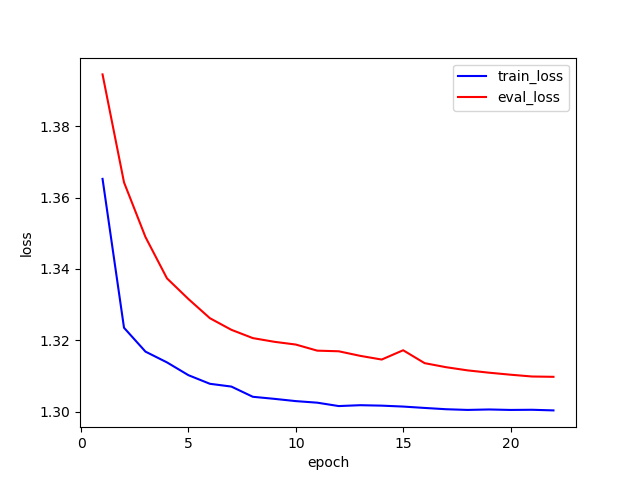
\includegraphics[width = .5\textwidth]{images/wine_loss.png}
	\caption{The epoch-loss curves for train data and validation data on wine-quality data set.}
	\label{fig:wine_loss}
\end{figure}

\subsection{Accuracy Rate of Two Data Set}
For iris data set, the hidden size is 64 with one hidden layer, batch size is 8, activator is \(tanh\) and learning rate is 0.01. The curve between iterations and loss value of train data set and validation set is show as Figure \ref{fig:iris_loss}. It is early stopped after training 69 iterations. The accuracy rate of train set, validation set and test set is respectively 98.33\%, 100\% and 100\%.

For wine-quality data set, the hidden size is 32 with two hidden layers, batch size is 16, activator is \(tanh\) and learning rate is 0.01. The curve between iterations and loss value of train data set and validation set is show as Figure \ref{fig:wine_loss}. It is early stopped after training 36 iterations. The accuracy rate of train set, validation set and test set is respectively 89.92\%, 90.37\% and 89.84\%.

We can see the fully connected Neural Network model performs well on nonlinear multi-classification problems, when the activator of output layer is \(softmax\) and the loss function is cross entropy. With proper depth of hidden layer and size of hidden layer, the loss value is near to zero and the accuracy rate is up to more than 90\%.

\subsection{Accuracy Rate of Different Hyper Parameters}
There are some hyper parameters affecting the performances of result, including depth of hidden layer, size of each hidden layer, batch size, activator and initialization of learnable parameters. We choose various values for each hyper parameter to evaluate the performances.

\textbf{Initialization method}. If the initial weights are full of zero. The accuracy rate on iris data is only around 50\%. The loss value decreases very slowly until number of iterations is around 500. Because when all weights are zero, the output of each layer is zero and the gradient delta of each layer is also zero except the  bias of output layer. So there is only a learnable parameter changing in the training which is the bias of the output layer. We can use random number in [-0.1, 0.1] or random number based normal distribution to initial parameters.

\textbf{Hidden layer size}. When the number of neurons of hidden layer increase, the accuracy increases first and then decreases. Because the model can not learn enough features from data set when the hidden size is too small. In comparison that, the model is easily overfitting and learn the features which is not universal but specific to this data set. So the hidden layer size should not be too big or too small.

\textbf{Batch size}.
When the bigger is the batch size from 8 to 128, the faster is the speed of each iteration. But more and more epochs are required to achieve the similar accuracy and even it can not achieve the similar accuracy, when the batch size is increasing. So the batch size should also not be too big or too small.

\section{Conclusion}
We implement the fully connected Neural Network based on Python and numpy, and train and evaluate model on two data sets including iris and wine-quality. The model has one input layer, one output layer, and multiple hidden layers. We use \(softmax\) activator and cross entropy cost function to solve the muti-classification problems. The accuracies on two data set are both bigger than 90\%.

But there are also some limitations in the current model. We only use the fully connected layer. But when the numbers of neurons and features is much larger, the speed of calculations will be very slow. We can use convolutional neural network when the number of neurons are larger.

What's more, if the depth of hidden layer is larger, the problems of gradient vanishing and gradient exploding will be easier to occur. We can use drop out mechanism to avoid them, that is, the model drops out randomly some neurons at each batch training and only optimize weights of the rest neurons. When predicting target value, the model use all the neurons to calculate the output.


\end{document}
